\chapter[piet-editorを作ったので宣伝]{piet-editorを作ったので宣伝}

周りの人がよくPietのエディタを作っているので
\footnote{Pietのエディタを作った話(\url{http://www.slideshare.net/KMC_JP/piet-46068527}) Pidet \url{https://github.com/dnek/Pidet}}
\footnote{Muratam/UltraPiet \url{https://github.com/Muratam/UltraPiet}}、
一度ぐらい作っておかないといけないかな と思って作りました。

\url{https://piet-editor.github.io/}です。
スマートフォンでもPietの実行ぐらいはできそうな感じですが、全ての機能を利用するにはPCから実行してください。

ブラウザで描いたり実行したり共有したりできるようにと作りました。
描く、実行、ステップ実行、

こんな感じの画面が出たりするはずです\footnote{画面は開発中のものです。大きな変更が入る可能性がありますが、何も出ないとか明らかなバグみつけたら教えてください……。}。
CSSをまだ全く書いていないので(あとデバッグ用の出力が下のほうに出ています)、まだUIがわかりづらいかもしれません。
\begin{center}
  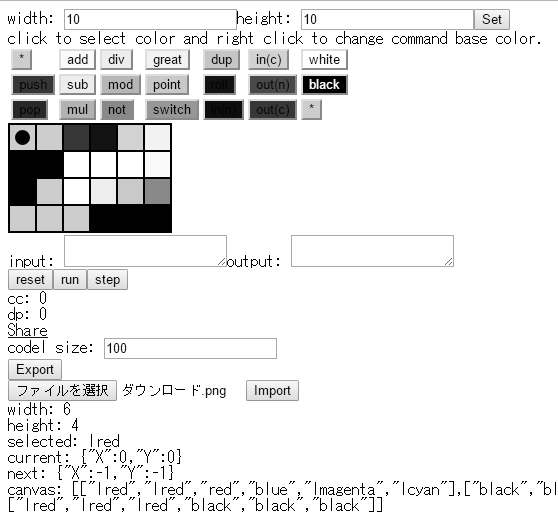
\includegraphics{images/editor_g.png}
\end{center}
